%%%%%%%%%%%%%%%%%%%%%%%%%%%%%%%%%%%%%%%%%
%
% (c) 2022 by Jennifer Laaser
%
% This work is licensed under the Creative Commons Attribution-NonCommercial-ShareAlike 4.0 International License. To view a copy of this license, visit http://creativecommons.org/licenses/by-nc-sa/4.0/ or send a letter to Creative Commons, PO Box 1866, Mountain View, CA 94042, USA.
%
% The current source for these materials is accessible on Github: https://github.com/jlaaser/pogil-polymers
%
%%%%%%%%%%%%%%%%%%%%%%%%%%%%%%%%%%%%%%%%%

\renewcommand{\figpath}{content/polymphys/mechanical-properties/elasticity/figs}
\renewcommand{\labelbase}{elasticity}

\begin{activity}{Elasticity of Polymer Networks}

\begin{instructornotes}
	This activity introduces students to concepts related to the tensile properties of polymer networks.
	
	After completing this activity, students will be able to:
	\begin{enumerate}
		\item Relate the macroscopic deformation of a polymeric material to deformation of individual chains
		\item Calculate the force that it takes to extend a polymer network along a single axis
		\item Express the force/extension relationship for a polymer network in terms of stress and strain
	\end{enumerate}
	
	\subsection*{Activity summary:}
	\begin{itemize}
		\item \textbf{Activity type:} Learning Cycle
		\item \textbf{Content goals:} See above
		\item \textbf{Process goals:} %https://pogil.org/uploads/attachments/cj54b5yts006cklx4hh758htf-process-skills-official-pogil-list-2015-original.pdf
			\begin{enumerate}
				\item Linking concepts to derive a key result
				\item Written and oral communication of reasoning
			\end{enumerate}
		\item \textbf{Duration:} 35-40 minutes, including time for class discussion
			\begin{itemize}
				\item If you are short on time, presenting the results from CTQs 1-3 in a mini lecture (or having students do these questions as a warm-up before class) and then having students start the activity at CTQ 4 also works well
			\end{itemize}
		\item \textbf{Instructor preparation required:} none beyond knowledge of relevant content
		\item \textbf{Related textbook chapters:}
			\begin{itemize}
				\item \emph{Polymer Chemistry} (Hiemenz \& Lodge), 2nd ed.: section 10.5
				\item \emph{Introduction to Polymers} (Young \& Lovell), 3rd ed.: section 21.3
			\end{itemize}
		\item \textbf{Instructor notes:}
			\begin{itemize}
				\item In Model 2, the given relationships for stress and strain are the engineering stress and engineering strain, not the true stress and true strain.
			\end{itemize}
	\end{itemize}
	
\end{instructornotes}


\begin{model}[Stretching a Piece of Polymer]
	\label{\labelbase:mdl:macrostretch}
	
	A simple model for the deformation of a macroscopic piece of a polymer is shown below:
	
	\vspace{6pt}
	\centerline{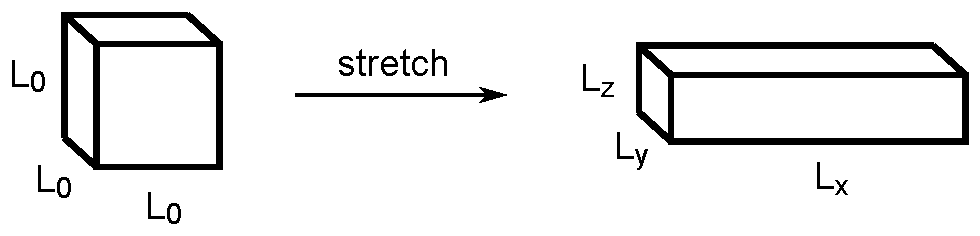
\includegraphics[width=0.7\textwidth]{\figpath/Model1_extension.pdf}}
	
	Usually, because we would like to look at properties that don't depend on the exact dimensions of the sample we are studying, we work in terms of the ratios of the final dimensions of the sample to its initial dimensions.
	
	For the sample shown above, the \emph{extension ratios} are:
	\begin{align*}
		\lambda_x = \frac{L_x}{L_0} && \lambda_y = \frac{L_y}{L_0} && \lambda_z = \frac{L_z}{L_0}
	\end{align*}
	These relationships allow us to write the final dimensions of the sample as
	\begin{align*}
		L_x = \lambda_x L_0 && L_y = \lambda_y L_0 && L_z = \lambda_z L_0
	\end{align*}
	
\end{model}


\begin{ctqs}

	\question First, consider the properties of the macroscopic sample.
	
		\begin{enumerate}
		
			\item What is the volume of the polymer sample depicted in Model \ref{\labelbase:mdl:macrostretch} before it is stretched?  Give your answer in terms of $L_0$.
	
		\begin{solution}[0.75in]{}
		
			$V = L_0^3$
		\end{solution}
	
			\item What is the volume of the polymer sample after it is stretched? Give your answer in terms of $L_x$, $L_y$, and $L_z$.
	
		\begin{solution}[0.75in]{}
		
			$V = L_x L_y L_z$
		\end{solution}
	
			\item There is usually no change in volume when we deform a bulk polymer network.  Write a mathematical relationship expressing this fact.
		\label{\labelbase:ctq:equalvolumes}
		\begin{solution}[0.75in]{}
			$L_0^3 = L_x L_y L_z$
		\end{solution}
			\item Use the information in Model \ref{\labelbase:mdl:macrostretch} to rewrite your the relationship from CTQ \ref{\labelbase:ctq:equalvolumes} in terms of $\lambda_x$, $\lambda_y$, and $\lambda_z$, and simplify as much as possible. \label{\labelbase:ctq:equalvolumes2}
	
		\begin{solution}[1.5in]{}
			\begin{align*}
				L_0^3 &= (\lambda_x L_0)(\lambda_y L_0)(\lambda_z L_0) \\
				L_0^3 & = \lambda_x \lambda_y \lambda_z L_0^3 \\
				1 &= \lambda_x \lambda_y \lambda_z
			\end{align*}
		\end{solution}
		
		\end{enumerate}
		
	\question The specific type of deformation illustrated in Model \ref{\labelbase:mdl:macrostretch} is an \emph{uniaxial} extension, in which the material is only stretched in one direction.
	
		Suppose we stretch the material in the $x$ direction by ratio $\lambda_x \equiv \lambda$.  
		
			\begin{enumerate}
				\item \emph{Qualitatively}, what must happen to the values of $\lambda_y$ and $\lambda_z$ to ensure that the volume of the material does not change?
				
					\begin{solution}[1in]{}
						Qualitatively, if the material is stretched along the $x$ direction, its dimensions in the $y$ and $z$ directions must decrease to maintain a constant volume.
					\end{solution}
				
				\item Assuming $\lambda_x \equiv \lambda$, find expressions for $\lambda_y$ and $\lambda_z$ (in terms of $\lambda$) that ensure that the relationship you derived in CTQ \ref{\labelbase:ctq:equalvolumes2} is satisfied.
		
				\emph{Hint: you may assume that $\lambda_y = \lambda_z$.}
				
					\begin{solution}[1.5in]{}
						\begin{align*}
							1 &= \lambda_x \lambda_y \lambda_z\\
							&= \lambda \lambda_y^2 \\
							\lambda_y^2 &= \frac{1}{\lambda}\\
							\lambda_y = \lambda_z &= \frac{1}{\sqrt{\lambda}}
						\end{align*}
					\end{solution}
				
			\end{enumerate}
	
	\question Finally, if the polymer strand initially has end-to-end vector $\vec h_0 = (x_0, y_0, z_0)$, what do you expect its final end-to-end vector $\vec h$ will be, if the polymer strand stretches by the same ratios that the macroscopic sample does?  \label{\labelbase:ctq:affinedef}
			
			\emph{(Note: this assumption, that the individual chains stretch by the same ratios as the macroscopic sample, is referred to as \emph{affine deformation}.)}
		
			\begin{solution}[0.75in]{}
				$\vec h = (\lambda x_0, \frac{y_0}{\sqrt{\lambda}}, \frac{z_0}{\sqrt{\lambda}})$
			\end{solution}
				
\end{ctqs}

\begin{infobox}

	As you have learned, when a single strand of polymer is stretched from end-to-end distance $h_0$ to end-to-end distance $h$, its change in entropy is 
			\begin{equation*}
				\Delta S_{strand} = -k_B\left(\frac{3}{2Nb^2}\right)(h^2 - h_0^2)
			\end{equation*}
	Combining this result with your answer to CTQ \ref{\labelbase:ctq:affinedef}, it is possible to show that under uniaxial deformation,
	
		\begin{equation*}	
				\Delta S_{strand} = -\frac{k_B}{2}\left(\lambda^2 + \frac{2}{\lambda} - 3\right)
			\label{\labelbase:eqn:delSstranduniaxial}
		\end{equation*}
			
\end{infobox}

\begin{ctqs}
		
	\question Suppose that there are a total of $v_e$ polymer strands that stretch when the material is stretched (we refer to these as ``elastically-effective'' strands). What will the total entropy change of the network ($\Delta S_{network}$) be, in terms of $v_e$, $\lambda$, and any other necessary constants?
		
			\begin{solution}[1.25in]{}
				\begin{align*}
					\Delta S_{network} &= v_e \Delta S_{strand}\\
						&= -\frac{v_e k_B}{2}\left(\lambda^2 + \frac{2}{\lambda} - 3\right)
				\end{align*}
			\end{solution}
		
	\question Finally, recalling that $f = -T\left(\frac{\partial S}{\partial L}\right)$, find an expression for the force required to stretch the material by extension ratio $\lambda$.
	
		\emph{Hint: Because $L = \lambda L_0$, we can also write $f$ as $f = -\frac{T}{L_0}\frac{\partial \Delta S}{\partial \lambda}$, which will be the easier form to use for this problem.}
		
			\begin{solution}[2.5in]{}
			
				\begin{align*}
					f &= -\frac{T}{L_0}\frac{\partial}{\partial \lambda} \left(-\frac{v_e k_B}{2}\left(\lambda^2 + \frac{2}{\lambda} - 3\right)\right)\\
						&= \frac{T}{L_0}\frac{v_e k_B}{2}\frac{\partial}{\partial \lambda} \left(\left(\lambda^2 + \frac{2}{\lambda} - 3\right)\right)\\
						&= \frac{v_e k_B T}{2 L_0}\left(2\lambda - \frac{2}{\lambda^2} \right)\\
						&= \frac{v_e k_B T}{L_0}\left(\lambda - \frac{1}{\lambda^2} \right)
				\end{align*}
			\end{solution}
	
\end{ctqs}

\begin{model}[Stress and Strain]

	In most experiments, we usually report our data in terms of the \emph{stress} and \emph{strain} on the material, which normalize the force (stress) and change in length (strain) to the initial dimensions of the sample.
	
	The stress and strain are defined as follows:
	\begin{align*}
		\text{stress:} && \sigma = \frac{\text{force}}{\text{initial cross-sectional area}} = \frac{f}{L_0^2} \\
		\text{strain:} && \epsilon = \frac{\text{change in length}}{\text{initial length}} = \frac{L-L_0}{L_0}
	\end{align*}
	where $L$ is the length of the material along the direction of deformation (i.e. $L = \lambda L_0$).
	
\end{model}

\begin{ctqs}

	\question Write an expression for the stress, $\sigma$, in terms of $v_e$, $\lambda$, $L_0$, and any other necessary constants.
	
		\begin{solution}[0.8in]{}
			\begin{equation*}
				\sigma = k_BT\frac{v_e}{L_0^3}\left(\lambda - \frac{1}{\lambda^2}\right)
			\end{equation*}
		\end{solution}

	\question Write an expression for the strain, $\epsilon$, in terms of $\lambda$ and any other necessary constants.
	
		\begin{solution}[0.8in]{}
			\begin{equation*}
				\epsilon = \frac{L-L_0}{L_0} = \frac{L}{L_0} -1 = \lambda - 1
			\end{equation*}
		\end{solution}
		
	\question Recall that polymers behave like springs.  Hooke's law states that the relationship between force ($f$) and deformation ($x$) of a spring follows $f=kx$, where $k$ is an appropriate spring constant.
	
		Propose an equivalent relationship for stress and strain, using the \emph{Young's Modulus}, $E$, in place of the spring constant.
		
		\label{\labelbase:ctq:sigmaEeps}
		
			\begin{solution}[0.5in]{}
			
				$\sigma = E\epsilon$
				
			\end{solution}
	
\end{ctqs}

\begin{infobox}
	For small deformations ($\lambda$ close to 1), it is possible to show that
	\begin{equation*}
		E \approx 3k_BT\frac{v_e}{V}
		\label{\labelbase:eqn:youngsmodulus}
	\end{equation*}
	where $v_e$ is the total number of elastically-effective strands, and $V$ is the volume of the sample.
\end{infobox}

\begin{ctqs}
	\question Will the material become easier or harder to stretch as temperature is increased?  Explain your group's reasoning in 1-2 complete sentences.
	
		\begin{solution}[1.5in]{}
			The solution will become more difficult to stretch as temperature is increased.  Increasing $T$ increases the Young's modulus, which effectively makes the polymer behave as a stiffer spring.
		\end{solution}
	
	\question In 2-3 complete sentences, propose an experiment that you could do to measure the number of elastically-effective chains per unit volume in an unknown polymer sample.
	
		\begin{solution}[1.75in]{}
		
			To measure the number of elastically-effective chains per unit volume, we could slowly stretch the material while measuring the required force.  We could then convert the measured force at each extension to a stress (and strain), and fit the data to a line.  The slope of this line would give us the Young's modulus, and we could then divide by $3kT$ to get the number of elastically-effective chains per unit volume.
		
		\end{solution}
\end{ctqs}


\begin{exercises}

	\exercise Experimentally, we find that the number of \emph{elastically-effective} strands in a polymer network is always smaller than the \emph{total} number of strands in the network.  Using your knowledge of the structural features of polymer networks, suggest at least one reason that this might be true.
	
		\begin{solution}{}
		Some strands in the polymer network may form loops, which will not stretch when the material is stretched.  These strands will not be elastically effective, making the number of elastically-effective strands smaller than the total number of strands in the network.
			
			Note: alternatively, students may answer in terms of dangling ends, or sol fraction; both of these are also appropriate answers to this question.
		\end{solution}
	
	%\exercise Derive expression for $\Delta S_{strand}$ for uniaxial extension
	
	%\exercise Derive expression for $E$ at low strain
	
	%\exercise analyze experimental tensile data to extract Young's modulus
	
	\exercise Often, it is more useful to think about polymer networks in terms of the average \emph{molecular weight between crosslinks} rather than the number of elastically effective strands per unit volume.
	
		\begin{enumerate}
			\item Suppose your polymer of interest has density $\rho$.  What is the total mass of a sample of volume $V$?
			
				\begin{solution}{}
				$\rho V$
				\end{solution}
			
			\item How many chains of molecular weight $M_x$ would be contained in a sample of volume $V$?  Give your answer in terms of the  number of individual chains, not just moles of chains.
			
				\begin{solution}{}
				$\frac{N_{av} \rho V}{M_x}$
					
					(note: $N_{av}$ is Avogadro's number)
				\end{solution}
			
			\item Assuming all of these chains are elastically effective (i.e. that the number you calculated in the previous part is equal to $v_e$), find an expression for the number of elastically effective chains per unit volume in terms of the polymer density, the molecular weight between crosslinks, and any other necessary constants.
			
				\begin{solution}{}
				$\frac{v_e}{V} = \frac{1}{V}\left(\frac{N_{av} \rho V}{M_x}\right) = \frac{N_{av} \rho}{M_x}$
				\end{solution}
		\end{enumerate}
		
	\exercise Derive the expression for the Young's modulus given on page \pageref{\labelbase:eqn:youngsmodulus} by doing the following:
		
		\begin{enumerate}
			\item Substitute appropriate expressions for $\sigma$ and $\epsilon$ into your equation from CTQ \ref{\labelbase:ctq:sigmaEeps} and rearrange to solve for $E$.
			
				\begin{solution}{}
					\begin{equation*}
						\sigma = k_BT\frac{v_e}{L_0^3}\left(\lambda - \frac{1}{\lambda^2}\right)
					\end{equation*}
					and
					\begin{equation*}
						\epsilon = \frac{L-L_0}{L_0} = \frac{L}{L_0} -1 = \lambda - 1
					\end{equation*}
					so
					\begin{equation*}
						E = \frac{\sigma}{\epsilon} = \frac{k_BT\frac{v_e}{L_0^3}\left(\lambda - \frac{1}{\lambda^2}\right)}{\lambda - 1}
					\end{equation*}
				\end{solution}
			
			\item Use L'H\^opital's rule to find the limit of this value as $\lambda \to 1$, and show that it yields the same expression that was given on page \pageref{\labelbase:eqn:youngsmodulus}.
			
				\begin{solution}{}
					\begin{align*}
						\lim_{\lambda\to 1} E &= k_BT\frac{v_e}{L_0^3} \lim_{\lambda\to 1} \frac{\lambda - \frac{1}{\lambda^2}}{\lambda - 1}\\
							&= k_B T\frac{v_e}{L_0^3} \lim_{\lambda\to 1} \frac{\lambda^3 - 1}{\lambda^3 - \lambda^2}
					\end{align*}
					If we simply substitute in $\lambda=1$, the fraction becomes $0/0$, which we can't evaluate.  Recalling that L'H\^opital's rule tells us that
					\begin{equation*}
						\lim_{x\to c} \frac{f(x)}{g(x)} = \lim_{x\to c} \frac{\frac{df}{dx}}{\frac{dg}{dx}}
					\end{equation*}
					we find
					\begin{align*}
						\lim_{\lambda\to 1} E &= k_BT\frac{v_e}{L_0^3} \lim_{\lambda\to 1} \frac{\frac{d}{d\lambda}\left(\lambda^3 - 1\right)}{\frac{d}{d\lambda}\left(\lambda^3 - \lambda^2\right)} \\
							&= k_BT\frac{v_e}{L_0^3} \lim_{\lambda\to 1} \frac{3\lambda^2}{3\lambda^2 - 2\lambda}\\
							&= k_BT\frac{v_e}{L_0^3} \lim_{\lambda\to 1} \frac{3\lambda}{3\lambda - 2}
					\end{align*}
				\end{solution}
				\begin{solution}{}
					This final expression no longer has a denominator that goes to zero if we substitute in $\lambda =1$, so doing so, we obtain
					\begin{align*}
						\lim_{\lambda\to 1} E &= k_BT\frac{v_e}{L_0^3}\frac{3}{3 - 2}\\
							&= 3k_BT\frac{v_e}{L_0^3}
					\end{align*}
					Finally, recalling that $V = L_0^3$, we obtain
					\begin{align*}
						\lim_{\lambda\to 1} E &= 3k_BT\frac{v_e}{V}
					\end{align*}
					as desired.
				\end{solution}
		\end{enumerate}
		
	%\question Derive G for shear strain
	
\end{exercises}


%\begin{problems}
%
%	\problem First exercise
%	\problem Second exercise
%	
%\end{problems}


	
\end{activity}